\titlespacing*{\subsection}{0pt}{1.0em}{0.3em}
\titlespacing*{\paragraph}{0pt}{1.0em}{0.3em}

본 절에서는 국가 간 상호의존성과 높은 시계열 변동성을 보이는 외환 시장 환경에 B--MTGNN 모델을 적용하여 환율 간 구조적 관계를 학습하고 환율 예측을 수행한 실증 분석 결과를 제시한다.

\subsection{실험 환경}
본 연구는 2011년 1월--2025년 12월(180개월)의 월별 데이터를 사용하였으며, 학습 구간은 2011년 1월--2023년 12월(156개월), 검증 구간은 2024년 1월--12월(12개월), 평가 구간은 2025년 1월--12월(12개월)로 분할하였다. 분석 대상 통화는 미국(US Trade Weighted Dollar Index), 한국(KRW), 일본(JPY)의 세 국가로 설정하였다. 모델 입력은 총 33개 환율, 특성공학 그리고 환율 및 거시경제 변수로 구성된 월별 다변량 시계열 데이터이며, 이는 3개의 환율 변수와 12개의 특성 공학(Feature Engineering) 변수 그리고 18개의 거시경제 변수로 이루어진다. 특성 공학 변수에는 각 통화의 수익률, 수익률의 시차 변수, 통화 간 수익률 차이, 그리고 통화 간 상관계수와 같은 시장 기반 파생 변수가 포함된다. 거시경제 변수는 각 국가의 거시경제 환경을 반영하기 위해 금리, 국내총생산(GDP), 소비자물가지수(CPI), 고용, 실업률, 무역수지로 여섯 가지 지표를 미국, 한국, 일본에 대해 각각 수집하여 총 18개 변수로 구성하였다. 국가별 시계열 데이터는 서로 다른 휴일제, 거시경제 지표 발표일 등으로 인한 시차를 가질 수 있다. 본 연구에서는 모든 시계열을 월별 기준으로 수집하고, 관측치가 존재하지 않는 구간에 대해서는 직전 관측치 기반 데이터를 대체하는 전진 채움 기법을 적용하여 데이터의 연속성을 확보하였다. 또한, 관측되지 않는 결측치는 모델 학습 시 해당 입력값의 영향을 배제하는 마스킹 기법을 통해 처리하여, 결측치 자체가 예측에 왜곡된 영향을 미치는 것을 방지한다. 이러한 변수 구성은 통화 가치에 영향을 미치는 실물경제 및 금융 요인을 동시에 반영하기 위한 것이다.
베이지안 그래프 신경망의 주요 하이퍼파라미터는 학습률 0.00015, Dropout 0.02, 은닉 차원 256, 학습 에폭 180으로 구성되었다. 

\subsection{실험 결과}
테스트 성능 평가는 Root Relative Squared Error(RRSE)를 기준으로 평가되었으며, 평가 구간에서의 예측 결과 시각화와 통계적 검증을 통해 모델의 성능을 보수적으로 검증하였다.

\paragraph{예측 모델 성능 평가}
표~\ref{tab:forecast_2026}는 평가 구간인 2025년 1월부터 2025년 12월까지에 대한 모델 예측 성능을 요약한 것이다. 일본 엔화(JPY)가 0.2832로 가장 낮은 RRSE를 기록하여 세 통화 중 가장 높은 예측 정확도를 보였으며, 한국 원화(KRW)는 0.3374, 미국 달러 지수(US Trade Weighted Dollar Index)는 0.5159로 나타났다. 다음으로 그림~\ref{fig:testing_fx_all}는 평가구간의 월별 환율 예측 결과를 시각적으로 나타낸 것이다. 각 그래프에서 파란색 실선은 실제 환율 추세, 보라색 점선은 모델이 예측한 값, 그리고 분홍색 음영 영역은 95\% 신뢰 구간을 의미한다. 미국 달러 지수의 경우 상반기에는 상승 추세가 나타났다가 하반기로 갈수록 점진적으로 하락하는 패턴이 관찰된다. 한국 원화 환율의 경우 연초 이후 상승 흐름이 나타난 뒤 중반 이후 비교적 완만한 상승세가 이어지는 패턴을 보인다. 일본 엔화 환율의 경우 상반기에는 하락 추세가 나타나고 이후 완만한 안정 구간이 형성되는 특징을 보인다. 모델은 이러한 장기적인 상승 추세를 비교적 정확하게 포착하고 있으며, 일부 시점에서 실제값과 예측값 사이의 편차가 존재하지만, 전반적인 추세 방향은 일관되게 유지되는 것을 확인할 수 있다. 그리고 하락 후 안정화되는 흐름을 비교적 잘 반영하고 있으며, 실제 환율 값이 대부분 신뢰 구간 내에 포함되어 예측 신뢰성이 유지되었다.

\begin{figure*}[!t]
\centering
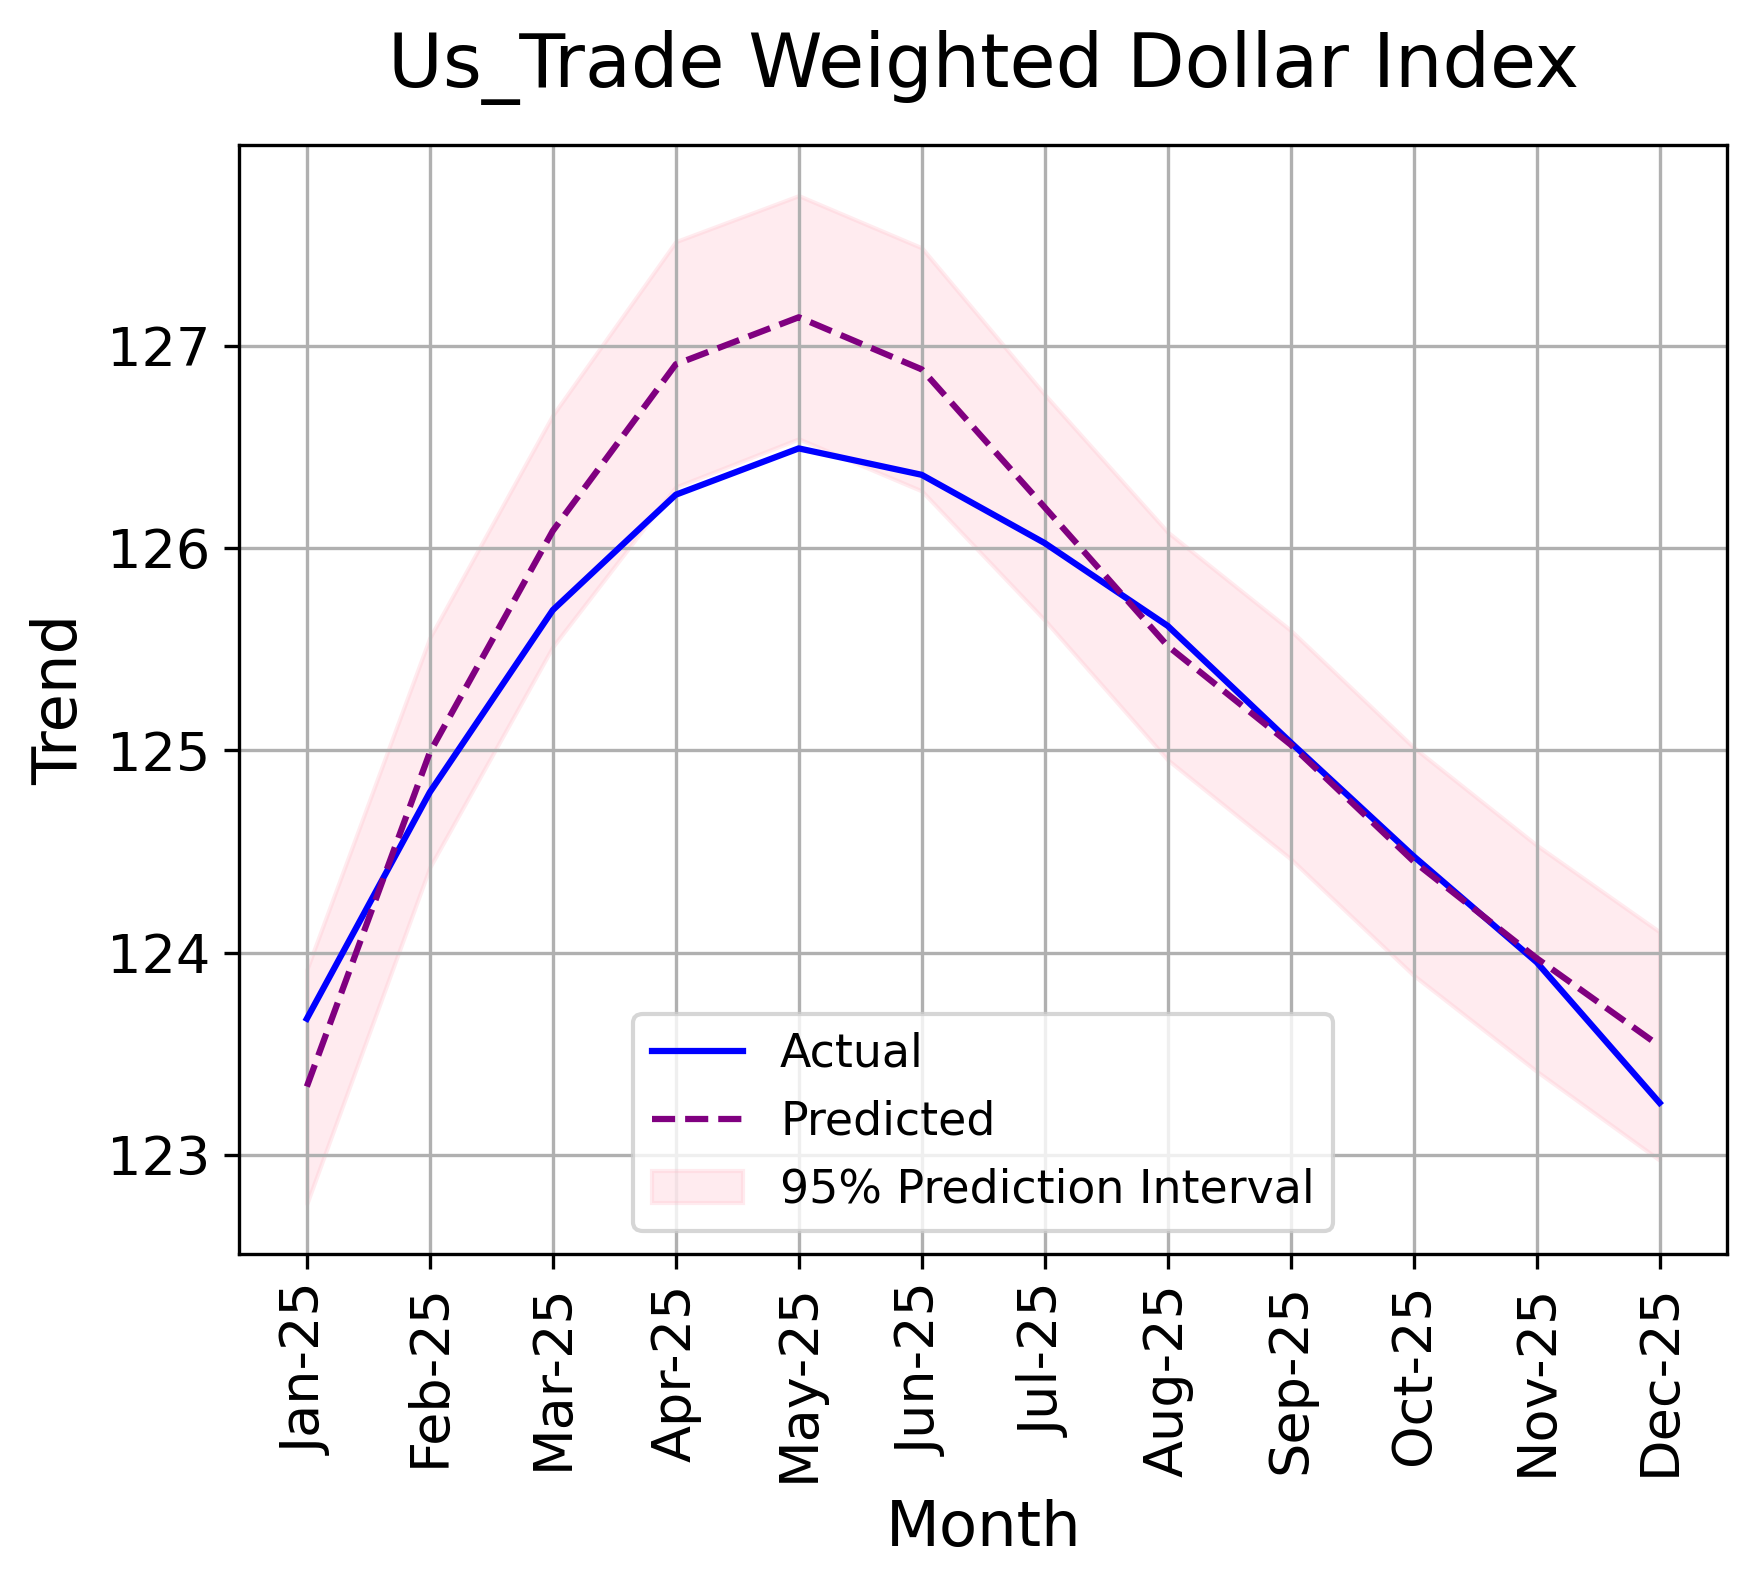
\includegraphics[width=0.32\textwidth]{figure/Us_Trade Weighted Dollar Index_Testing.png}
\hfill
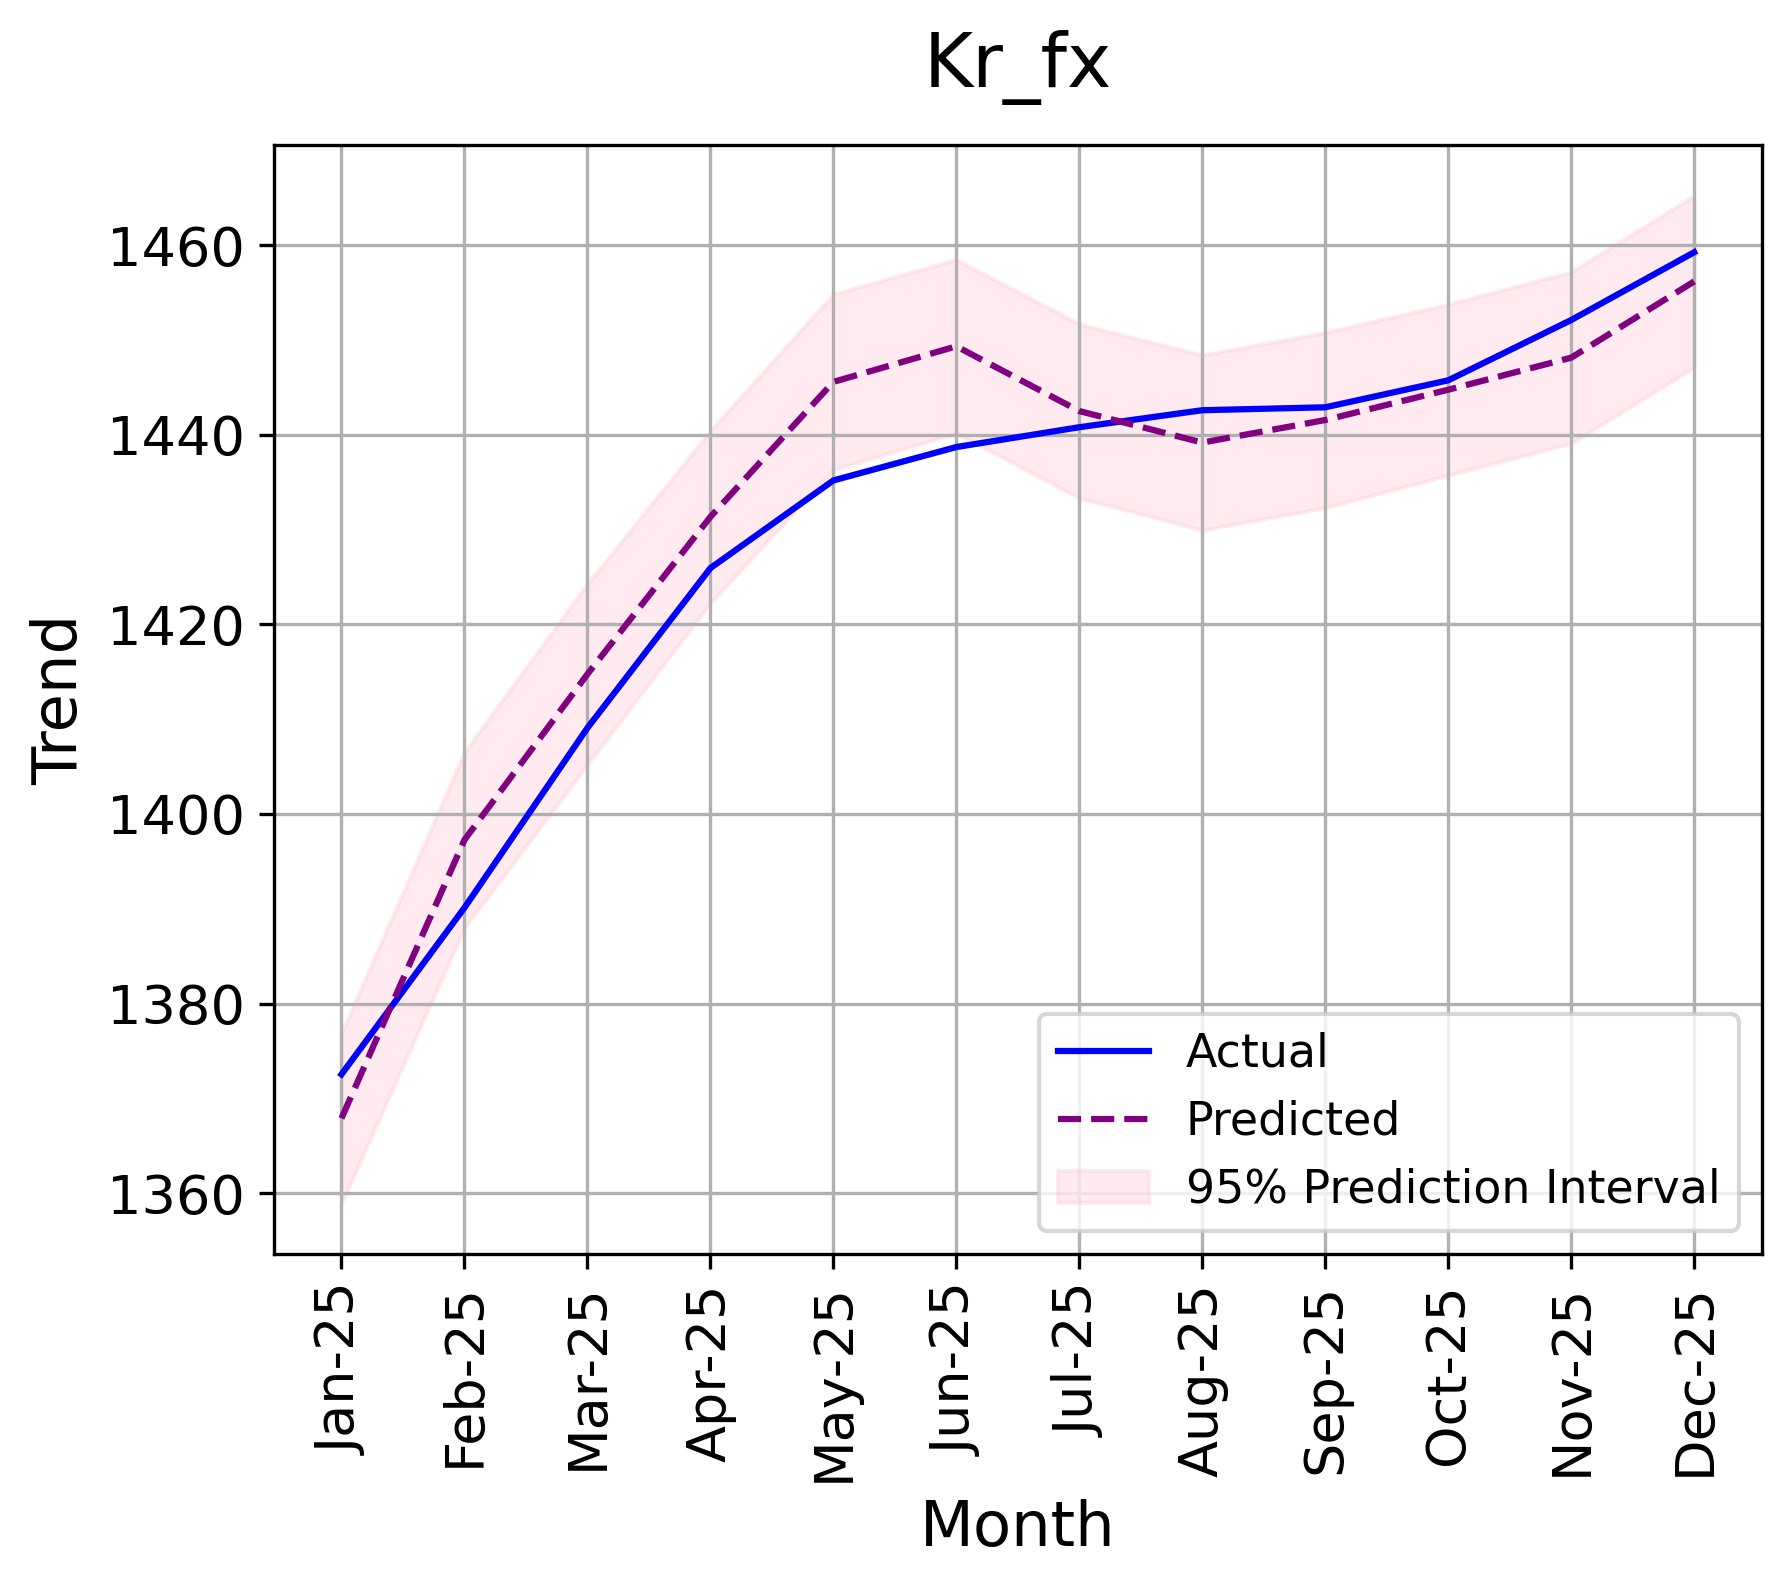
\includegraphics[width=0.32\textwidth]{figure/Kr_fx_Testing.png}
\hfill
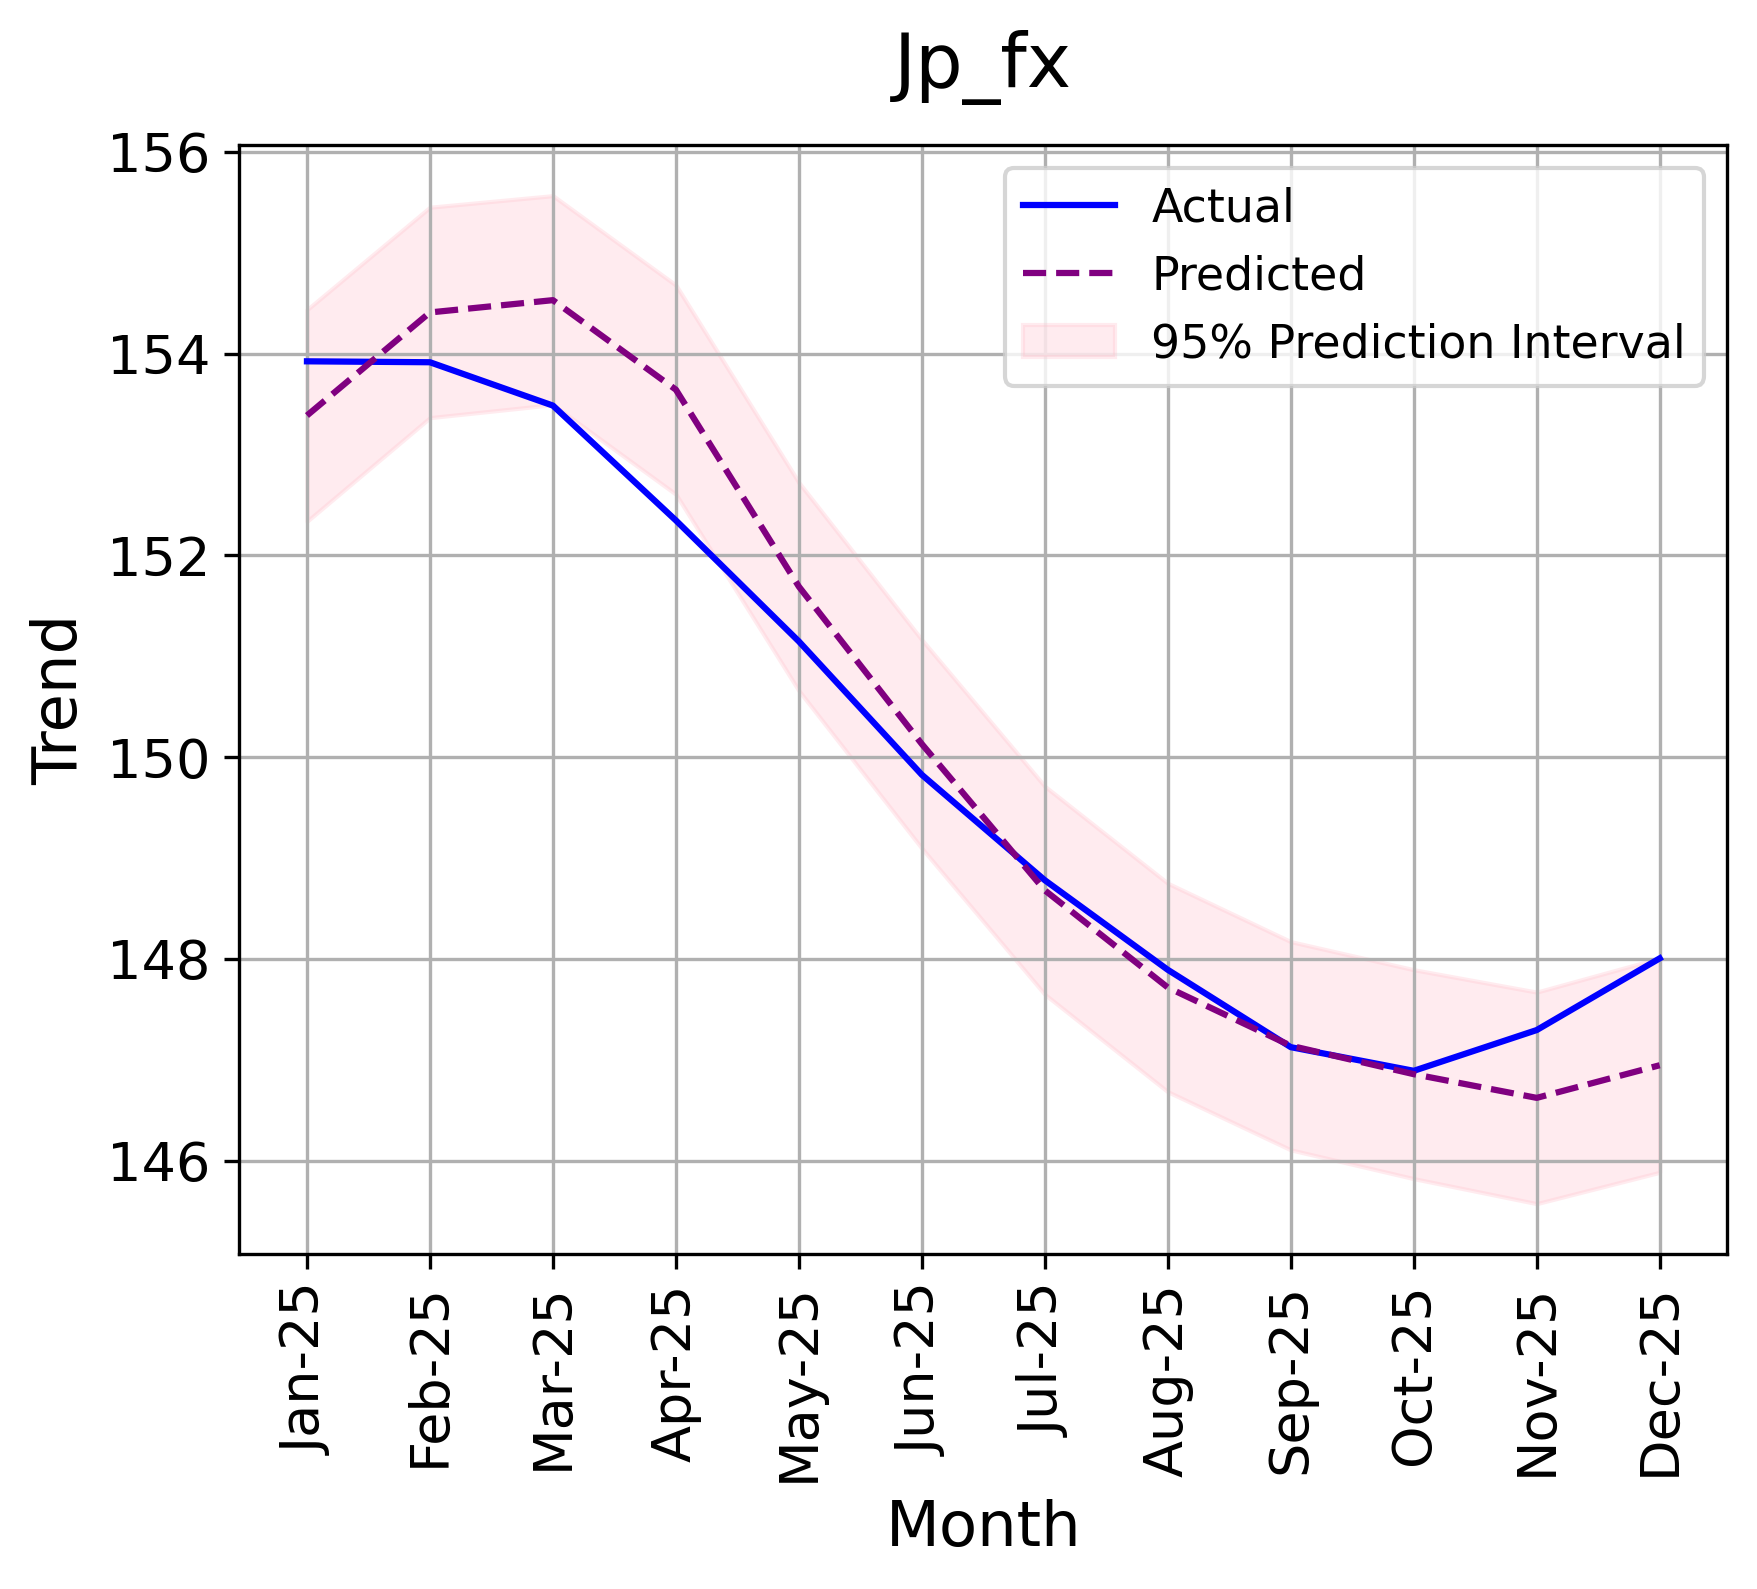
\includegraphics[width=0.32\textwidth]{figure/Jp_fx_Testing.png}
\caption{B--MTGNN 평가구간 성능 검증(좌 : US, 중 : KR, 우 : JP)}
\label{fig:testing_fx_all}
\end{figure*}

\paragraph{2026년 전망 및 결과}
2025년 12월까지의 관측값을 모델 학습으로 활용하여 2026년 1월--12월에 대한 환율 전망을 예측하였다. 표~\ref{tab:forecast_2026}는 MC dropout의 반복 횟수를 20회로 확대하여 생성한 베이지안 예측을 요약한 결과이며, 예측 평균과 95\% 신뢰 구간을 제시한다. 그림~\ref{fig:forecast_2026_normalized}에서도 확인할 수 있듯이, 국가 간 환율 경로는 예측 구간에 따라 국가 조합별로 상이한 변동 구조 패턴이 관측되었다. 2026년 말 기준 예측값을 살펴보면 미국 달러 지수는 약 121--122 수준으로 예측되었으며, 예측 구간은 약 117.90--118.99 범위로 나타났다. 일본 엔화는 약 153 수준으로 예측되었으며, 예측 구간은 약 159.44--207.44 범위로 추정되었다. 한국 원화 환율은 약 1,470--1,480원 수준으로 예측되었으며, 예측 구간은 약 1,457.29--1,490.76 범위로 나타났다. 특히 일본의 경우, 예측 구간 진입과 동시에 급격히 상승하며 신뢰구간의 폭 또한 비약적으로 확대되는 패턴이 관측되었다. 반면, 미국은 소폭 하락하며 수렴하는 양상을 보였고, 한국은 좁은 신뢰구간을 유지하며 상대적으로 안정적인 경로를 형성하였다.

\begin{figure*}[!ht]
\centering
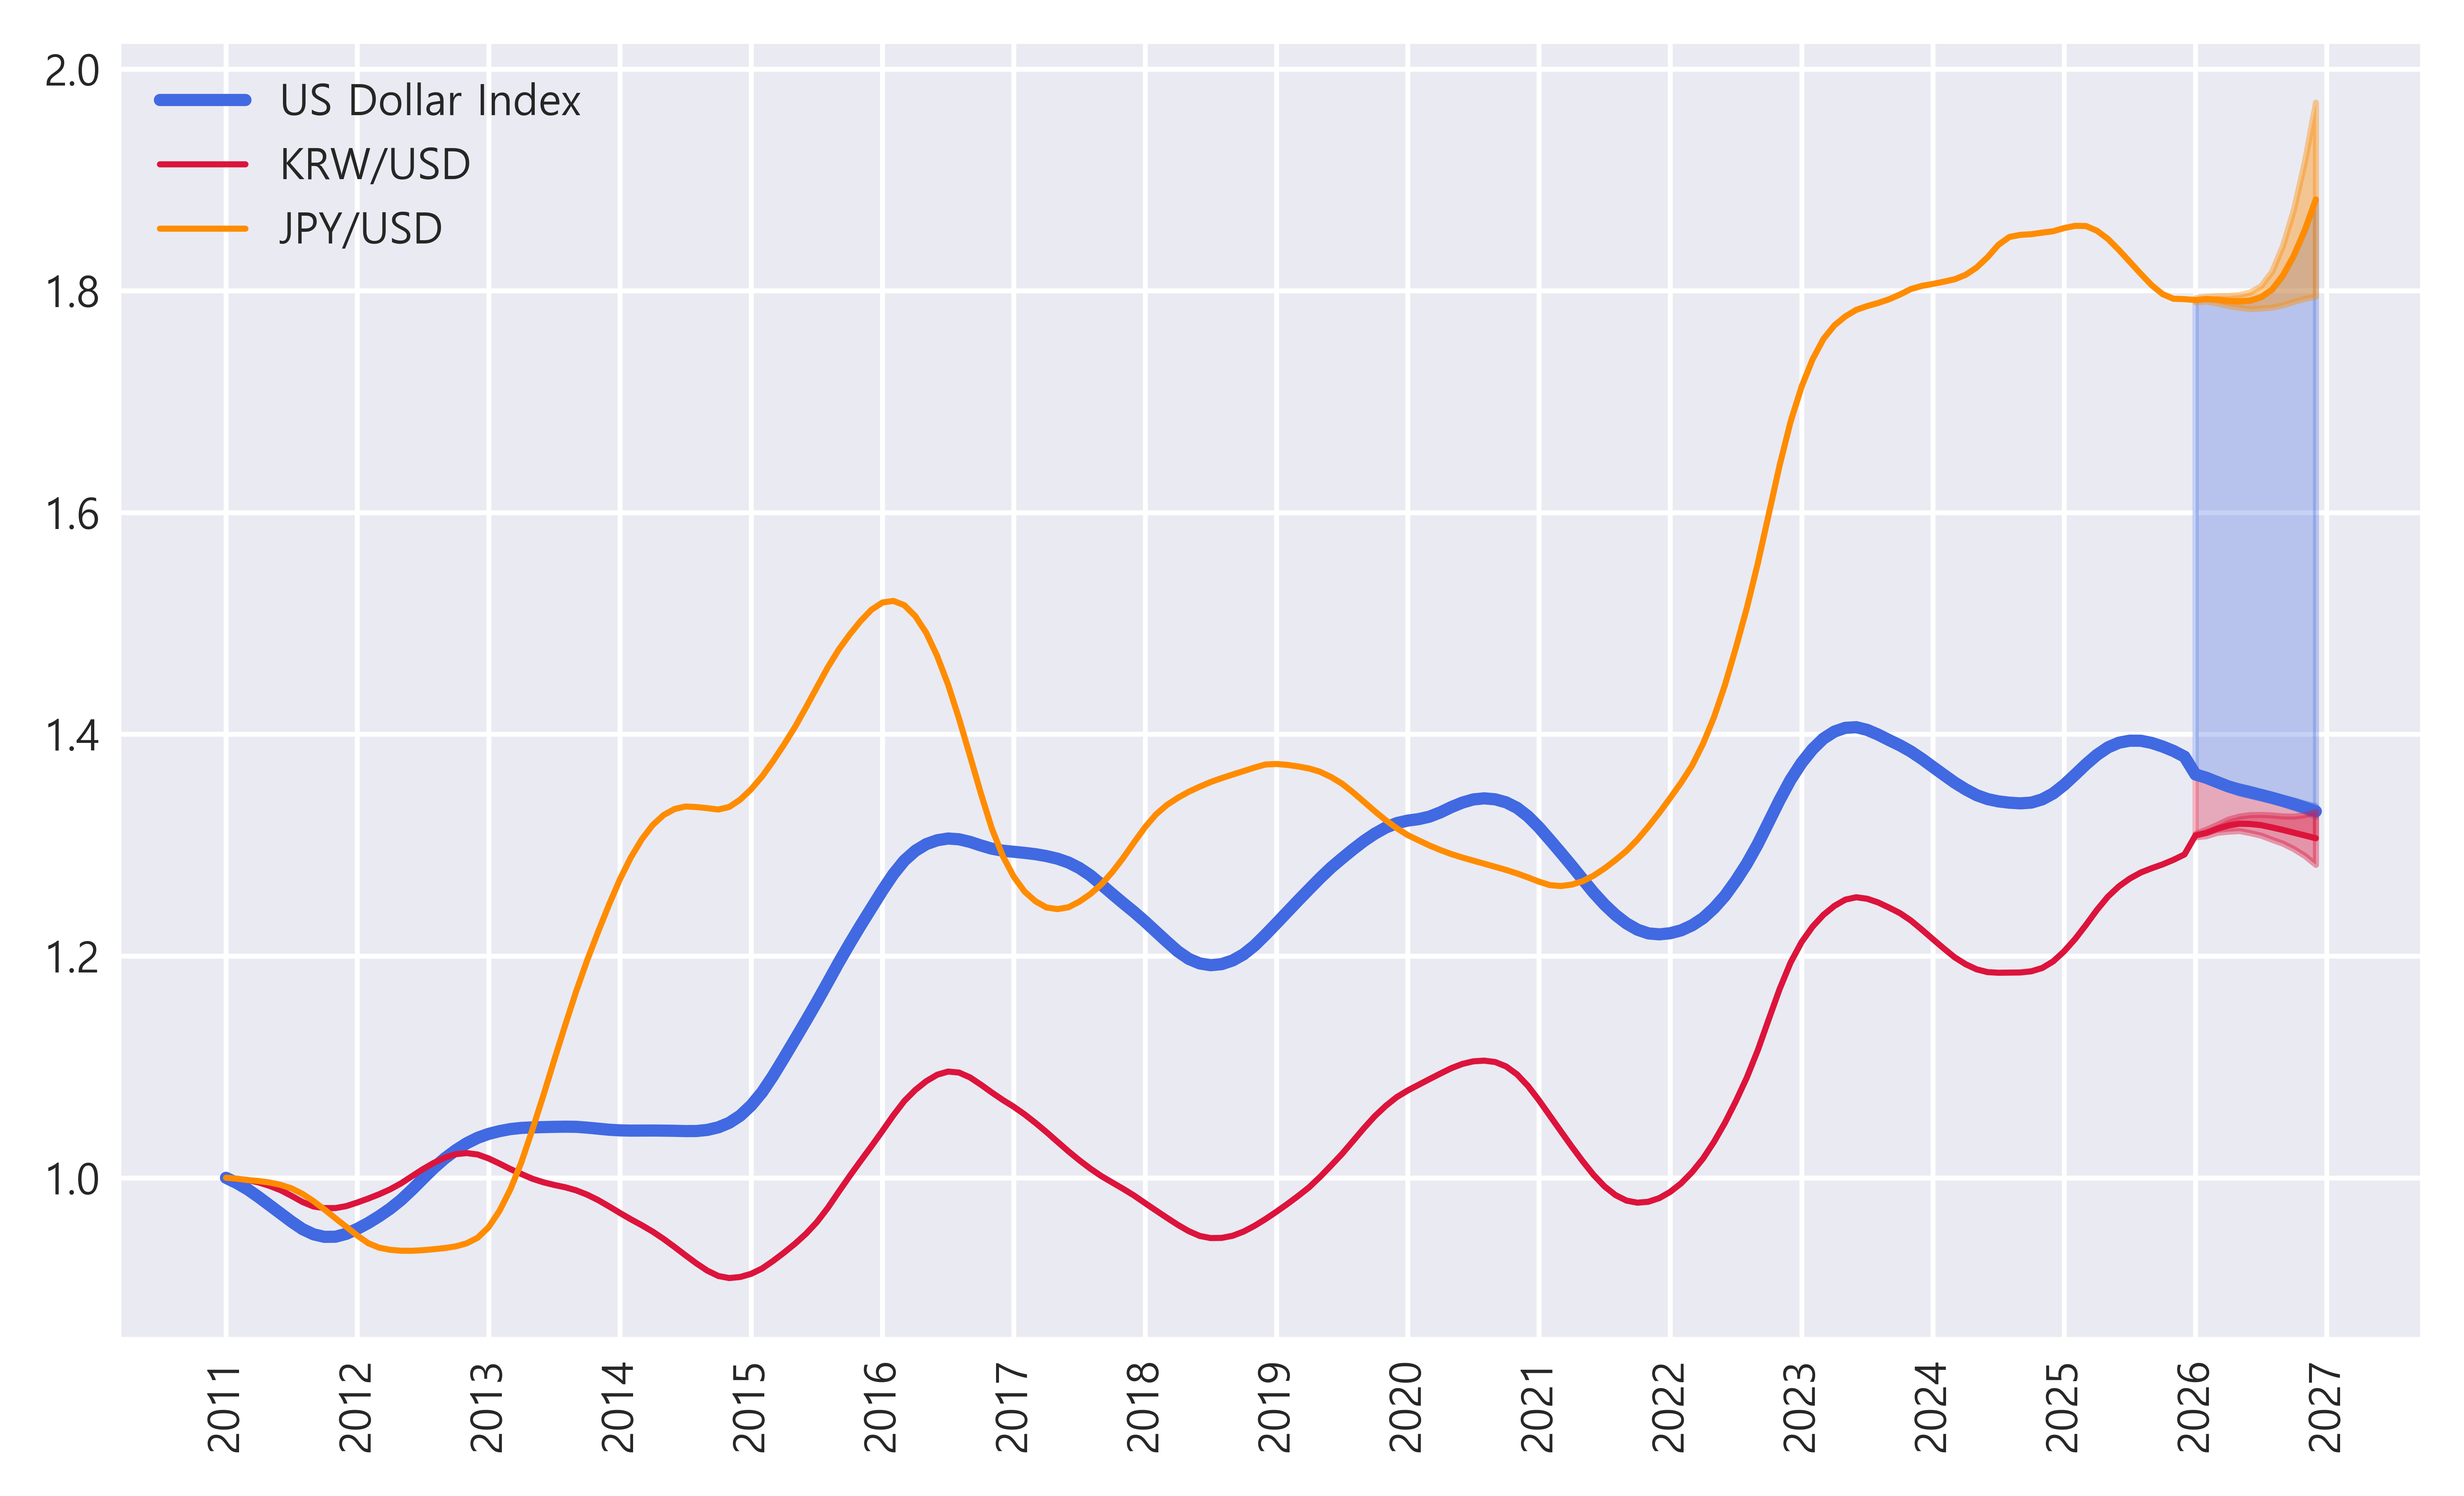
\includegraphics[width=\textwidth]{figure/Multi-Country Forecast Height Adjustment.png}
\caption{2026년 다중 통화 예측 경로(정규화). US Dollar Index와 KRW/USD 및 JPY/USD의 트렌드 예측 결과를 제시한다. 트렌드 플롯의 기간은 2011년 1월부터 2026년 12월까지이며, 이 중 2026년 1월부터 2026년 12월까지는 B--MTGNN 모델을 활용해 예측되었다. 환율 격차(Gap)는 해당 국가 환율 곡선과 동일한 색으로 강조되어 시각화되었다. 각 트렌드 예측에 대해서는 95\% 신뢰 구간이 함께 제시되어 있다. 각 환율 예측은 normalised 된 값이고 1.0은 정규화 기준점을 의미한다}
\label{fig:forecast_2026_normalized}
\end{figure*}

\begin{table}[t]
\centering
\caption{평가 구간 성능 및 예측 구간 요약}
\label{tab:forecast_2026}
\small
\setlength{\tabcolsep}{4pt}
\begin{tabular}{lccc}
\toprule
국가 & 성능검증$^{*}$ & 95\% 하한 & 95\% 상한 \\
\midrule
US (TWDI) & 0.5159 & 117.90 & 118.99 \\
JP (JPY)  & 0.2832 & 159.32 & 207.45 \\
KR (KRW)  & 0.3374 & 1457.29 & 1490.77 \\
\bottomrule
\multicolumn{4}{l}{\footnotesize $^{*}$성능검증평가: RRSE (Root Relative Squared Error)}
\end{tabular}
\end{table}

\paragraph{국가 간 예측 패턴 비교}
표~\ref{tab:gap_2026}은 2026년 예측된 환율 경로를 기반으로 국가 간 평균 수준 격차를 비교한 결과를 나타낸다. 각 값은 2026년 12개월 예측값을 평균하여 계산한 연간 평균 환율 차이로 정의된다. 분석 결과 일본--한국 조합이 0.637로 가장 큰 평균 격차를 보였으며, 일본--미국 조합은 0.61로 그다음으로 나타났다. 반면 미국--한국 조합은 0.026으로 상대적으로 작은 차이를 보였다. 이러한 결과는 세 국가 환율이 동일한 방향으로 움직이기보다는 국가별로 서로 다른 변동 경로와 조정 속도를 보일 가능성을 시사한다.

\begin{table}[t]
\centering
\caption{국가 간 상대적 환율 격차}
\label{tab:gap_2026}
\small
\setlength{\tabcolsep}{3pt}
\begin{tabular}{lc}
\toprule
국가 조합 & 평균 환율 격차 \\
\midrule
US--KR & 0.026 \\
JP--US & 0.610 \\
JP--KR & 0.637 \\
\bottomrule
\end{tabular}
\end{table}
\begin{figure}[!t]
\centering
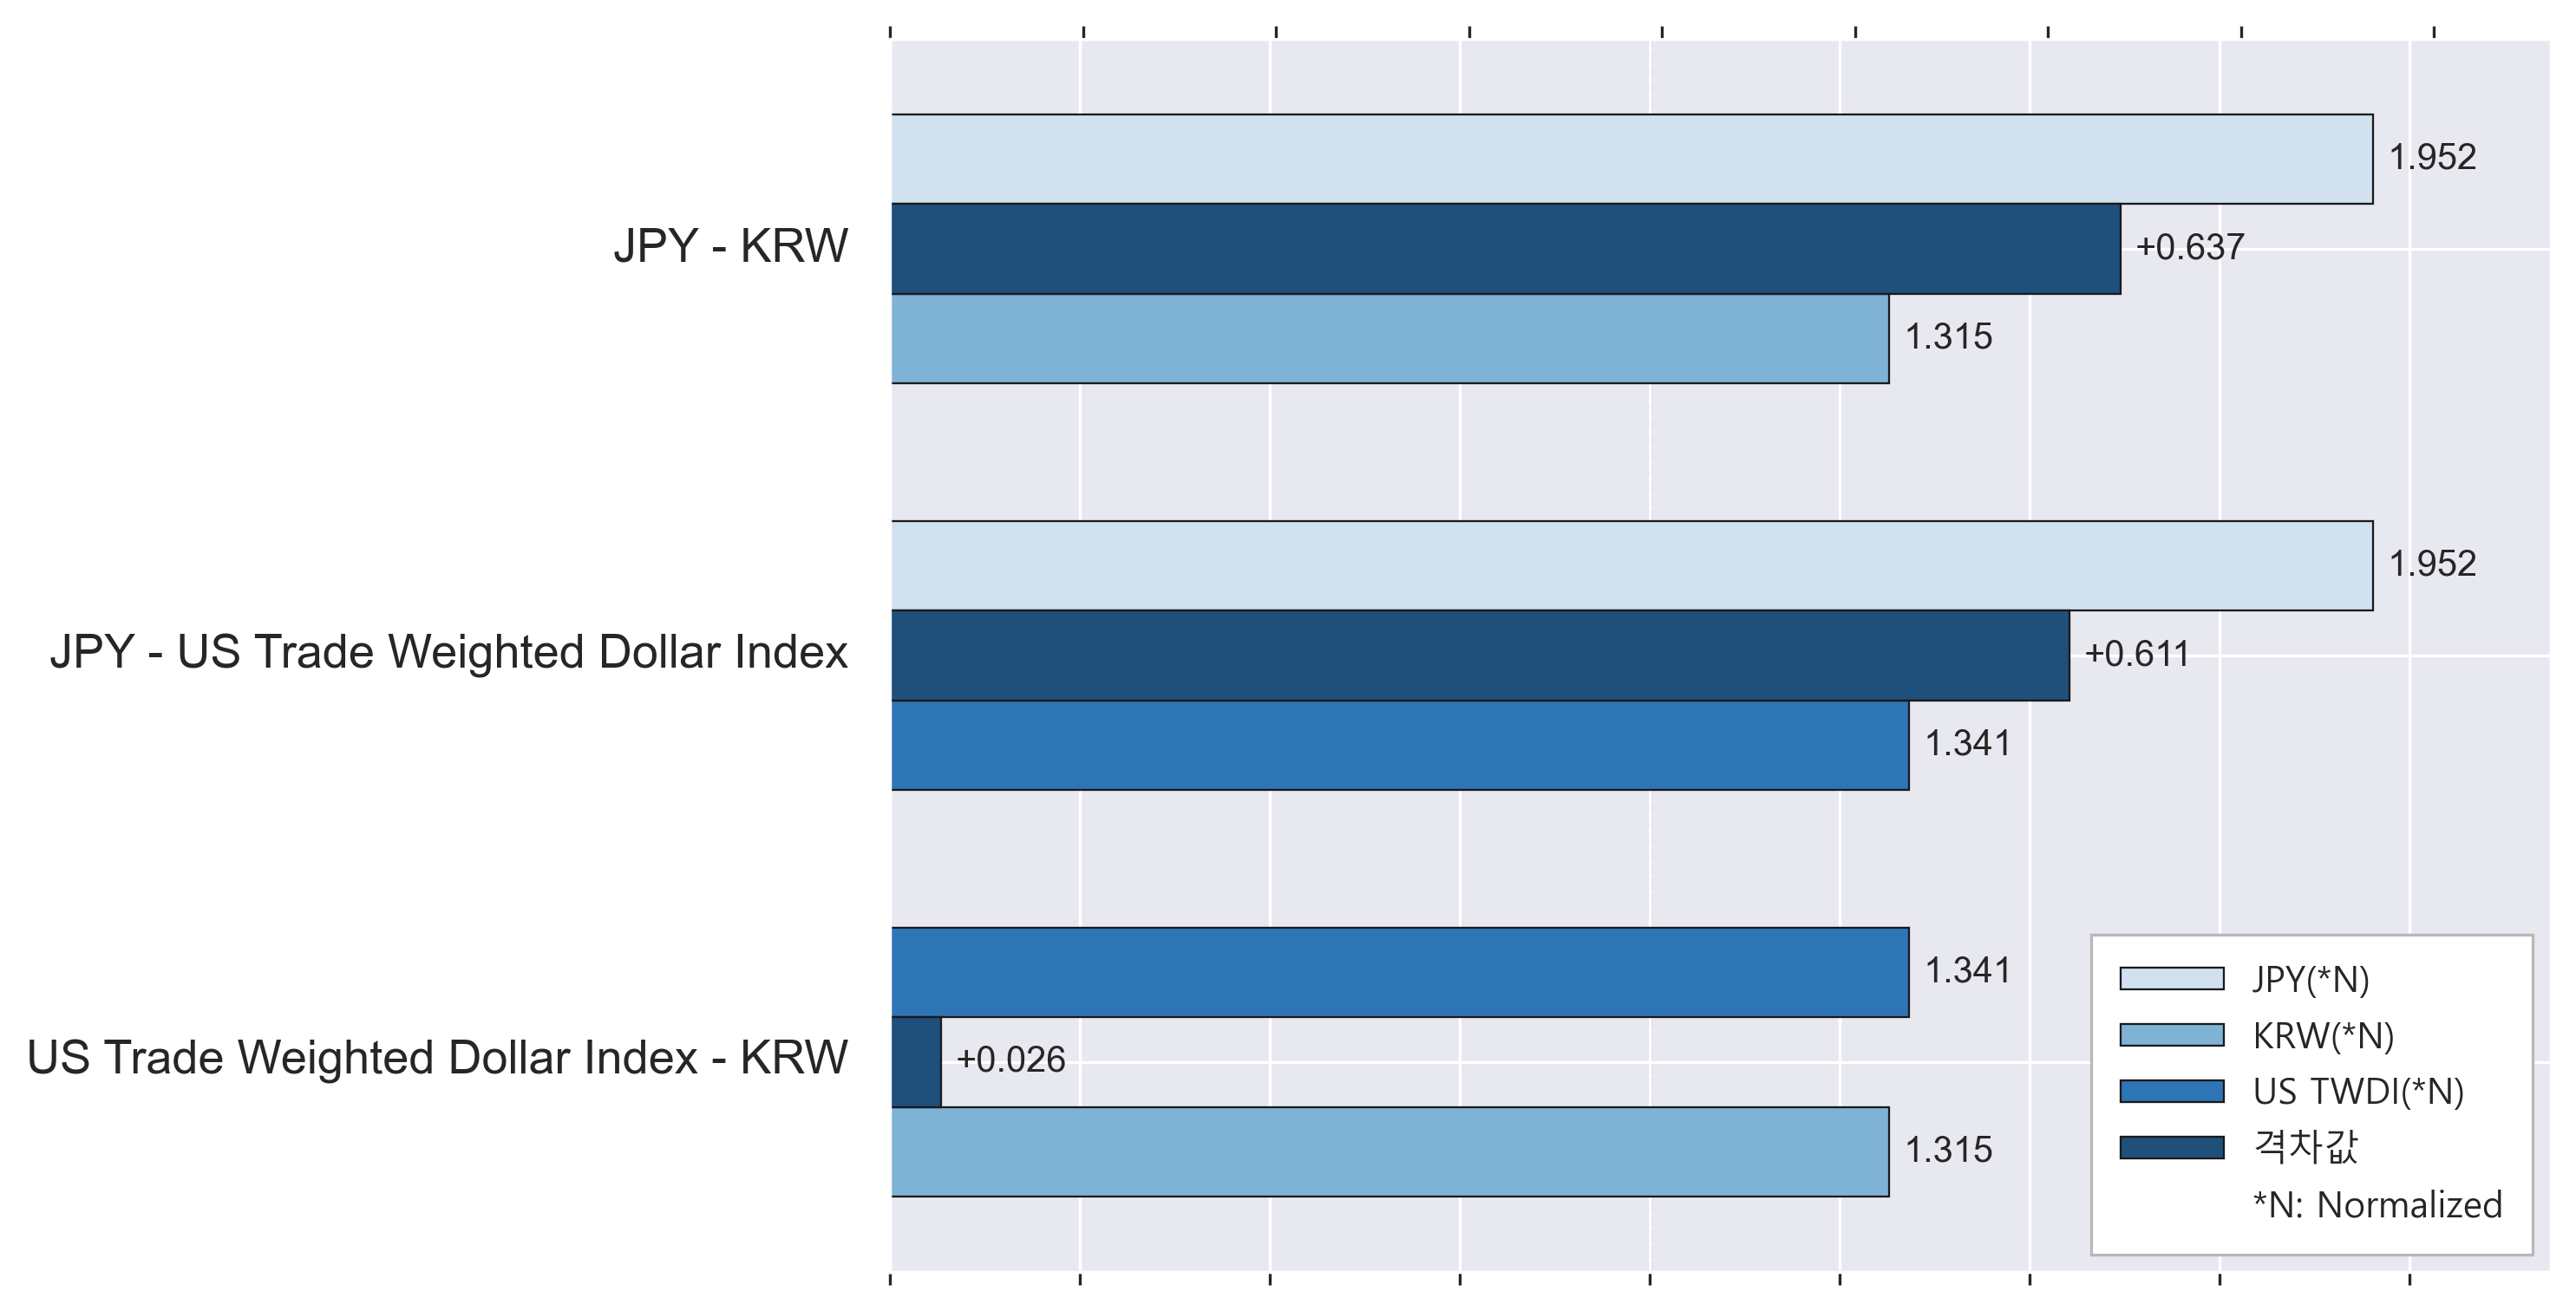
\includegraphics[width=\columnwidth]{figure/normalized_gap_bar_final.png}
\caption{국가 간 환율 격차($\mathrm{Gap}_{i,j}$) 비교}
\label{fig:normalized_gap_discussion}
\end{figure}

\paragraph{예측 모델 성능 연구 결과}
종합적으로 보았을 때, 제안한 B-MTGNN 모델은 국가 간 경제 변수와 환율 간 상호 관계를 반영하여 주요 환율의 추세 변화를 안정적으로 추정하는 모습을 보인다. 또한 베이지안 추론을 통해 예측값뿐 아니라 예측 불확실성을 함께 제공함으로써 금융 시계열 예측에서 중요한 위험 범위 정보를 동시에 제시할 수 있음을 확인하였다. 대부분의 실제 관측값이 95\% 예측 구간 내에 포함되어 예측 분포가 실제 변동성을 합리적으로 포착하고 있음을 확인하였다. 특히, 2025년 예측 평가 구간은 베이지안 추론을 통해 모델이 추정한 예측 불확실성을 반영한 것으로, 환율 변동 가능성이 존재하는 범위를 함께 제시한다는 점에서 단일 점 예측보다 해석적 가치가 있다. 정량적 예측 결과는 다르지만, 수치 출력만으로는 통화 전반의 패턴과 기본 경제 상황은 여전히 추론하기 어렵다. 본 연구는 예측된 내용에 대한 해석 가능한 설명을 제공하여 제안된 다중 에이전트 추론 프레임워크를 사용해 예측 결과를 추가로 분석하였다.

\subsection{2026년 예측에 대한 다중 에이전트 해석 결과}
표~\ref{tab:forecast_2026}와 표~\ref{tab:gap_2026}에서 확인된 정량적 환율 예측 결과와
점진적으로 증가하는 불확실성 구간의 원인을 검증하기 위해, 앞서 제안한 다중 에이전트 시스템에 예측 모델의 관측값, 예측값, 베이지안 불확실성에 대한 결과 데이터를 입력으로 주어 분석 결과를 도출하였다. 2026년에 대해 모델이 예측한 해당 에이전트의 해석 결과는 다음과 같다.

\paragraph{비선형적 신뢰구간 확장의 분석}
2026년 하반기로 진입할수록 모델의 95\% 신뢰구간과 CI 폭/평균 비율이 시간에 비례하여 급격히 확장되는 현상을 발견하였다. 이는 경제 정책 불확실성의 누적을 야기한다 \cite{Baker2016}. 에이전트는 이를 수학적 불확실성 구간으로 식별하고 단순한 통계적 노이즈가 아니라 특정 이벤트가 내재한 것으로 해석하였다. 이러한 변동은 미국의 관세장벽 본격화, 미·중 패권 경쟁 심화에 따른 반도체 공급망 통제, 지중해 및 중동발 원유 가격 급등과 같은 외생적 요인이 환율 변동에 영향을 미쳤을 가능성을 시사한다\cite{Caldara2022}.

\paragraph{원화(KRW)와 엔화(JPY)의 약세}
표~\ref{tab:forecast_2026}에서 평균 원화가 1,478.56원, 엔화는 151.26엔으로 약세 추세를 보인다. 에이전트 기반 분석에 따르면, 미국 연방준비제도(Fed)와 아시아 주요 중앙은행간의 정책 차이를 원인으로 지목하였다. 연준의 점진적 금리 인하 속도에 비해, 한국은행(BOK)의 물가 안정 중시 기조는 원화의 하락 경직성으로 연결되며, 일본은행(BOJ)의 실질 금리의 상승과 지속적인 완화적 상태가 구조적 약세를 형성하였다. 이러한 정책의 비대칭적 변화는 Miranda-Agrippino and Rey (2020)가 규명한 세계적 금융 주기와 일치하며~\cite{MirandaAgrippino2020}, 이러한 개별 국가의 정책 변화가 결과적으로 환율 약세로 발현되었다고 평가하였다.

\paragraph{달러 인덱스(TWDI)의 구조적 강세}
미국 무역가중달러인덱스(TWDI)의 경우, 통계 예측 모델은 점진적 하락세로 예측하였다. 그러나 2026년 평균 121.71이라는 타국 대비 견고한 높은 수준을 지속하는 현상에 대해, 에이전트는 미국의 상대적으로 견고한 경제 성장세 지속, 서비스 무역의 흑자, 그리고 지속적으로 높은 수준의 실질 금리 차이가 구매력 평가(Purchasing Power Parity, PPP) 및 금리평형(Interest Rate Parity, IRP) 이론이 달러의 강세를 지지한다고 분석하였다. 나아가 글로벌 무역의 분절화와 타국 통화들의 약세 환경이 전 세계의 안전자산 수요를 달러로 집중시키는 현상이 리스크 심화 요인으로 분석하였다. 이처럼 정량적 예측과 거시경제 간의 상황을 명시적으로 식별해 낸 것은 심층적인 학술적 해석 가능 역량을 지니고 있음을 증명한다.

이와 같은 멀티 에이전트 기반 해석 결과는 예측값 자체의 정확성을 직접적으로 평가하기보다는, 해당 결과가 시사하는 구조적 의미와 정책적 해석 가능성을 제시하는 데 목적이 있다. 이에 대한 더 깊이 있는 해석은 다음 장에서 추가로 논의한다.
